\section{Introduction to Bayesian Optimization}
%----------------------------------------------------------------------
\begin{frame}[c]{Introduction to Bayesian Optimization}
\framesubtitle{Global Optimization}

Consider a \emph{well behaved} function $\func$ : $\pcs \rightarrow \realnum$ where $\pcs \subseteq \realnum^D$ is a bounded domain. Our goal is to find
%
\begin{equation*}
  \optconf=\argmin_{\conf\in\pcs} \func(\conf).
\end{equation*}
\vspace{-0.6cm}

\begin{columns}[T]
\column{0.4\textwidth}
\begin{itemize}
    \item Function $\func$ is explicitly unknown - this is called a black box function
    \item and can be multimodal
    \item Only mode of interaction: Query $\conf$ to obtain a potentially noisy observation $\cost(\conf) = \func(\conf) + \epsilon$
    \item Evaluations are expensive
    \item There is no gradient information available
\end{itemize}
$\rightarrow$ For the remainder of this lecture we will \emph{minimize} $\cost$
%
\column{0.6\textwidth}
\begin{figure}
   \begin{multicols}{2}
    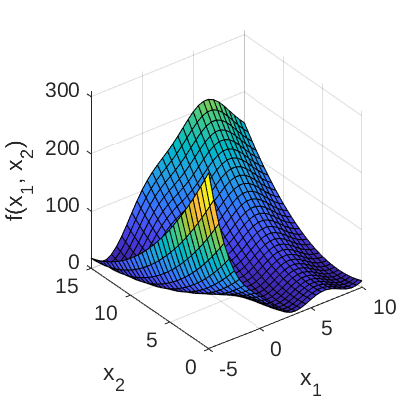
\includegraphics[width=0.4\textwidth, right]{images/intro_images/branin.png}
    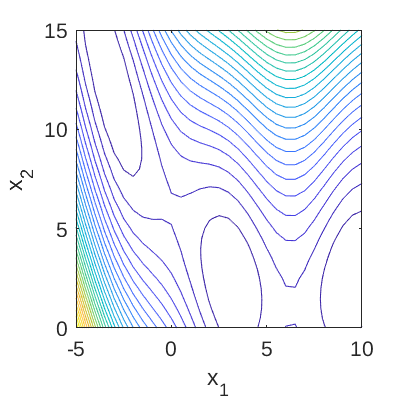
\includegraphics[width=0.4\textwidth,left]{images/intro_images/branin_countour.png}
 \end{multicols}
\end{figure}
\source{\href{https://uqworld.org/t/branin-function/53}{Branin}}
\end{columns}
\end{frame}
%----------------------------------------------------------------------
%\begin{frame}[c]{Optimization problem example}

%We know that:
%\begin{itemize}
%    \item The function $\cost$ is Lipschitz continuous and differentiable.
%    \pause
%    \item The minimizer of $\cost$ is in the interval [0,1].
%    \pause
%    \item We have observed 3 evaluations of $\cost$.
%\end{itemize}

%\end{frame}
%----------------------------------------------------------------------
%\begin{frame}[c]{Problem description}
%\framesubtitle{We have 4 function evaluations}
%\begin{figure}
%    \centering
%    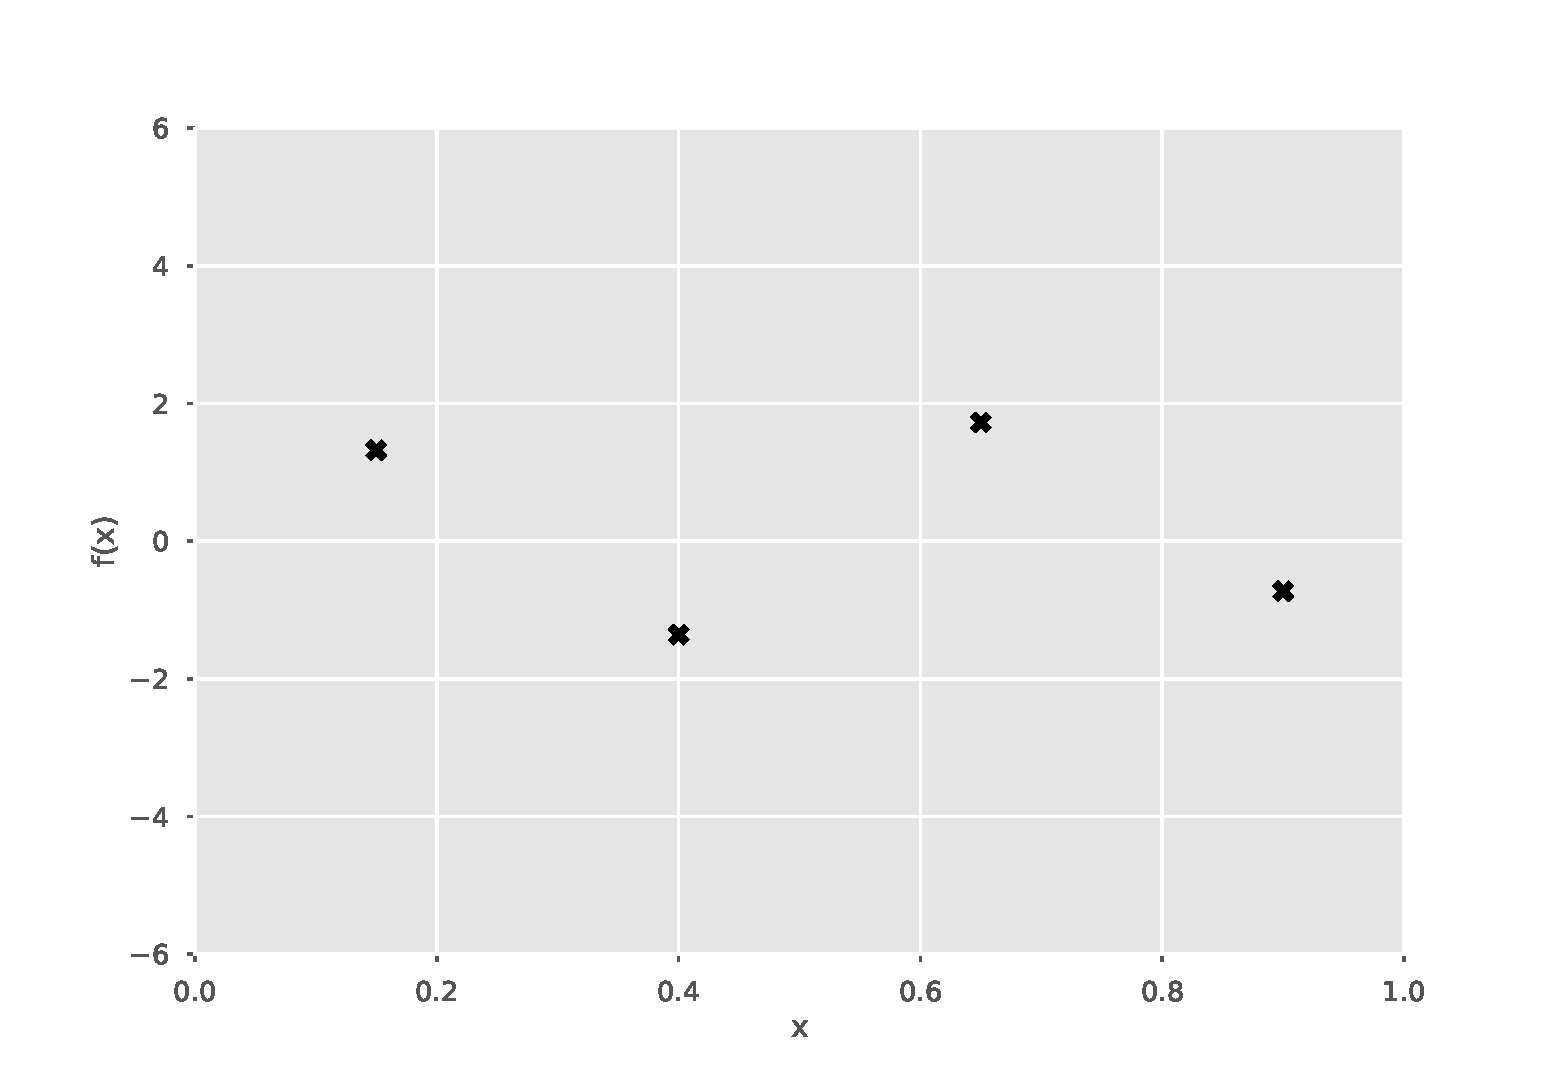
\includegraphics[width=0.8\textwidth, %height=0.38\textwidth]{images/intro_images/plot_datapoints.p%df}
%    \label{fig:my_label}
%\end{figure}
%\begin{center}
%  Where is the minimum of function $f$?  
%\end{center}
%\source{Plots are based on Javier Gonz\'alez's BO lecture %(bo\_intro.py)}



%\end{frame}

%-----------------------------------------------------------------------
%----------------------------------------------------------------------
%\begin{frame}[c]{Problem description}
%\framesubtitle{One possible curve}
%\begin{figure}
%    \centering
%    \includegraphics[width=0.7\textwidth, %height=0.4\textwidth]{images/intro_images/plot_posterior_1_s%ample.pdf}
%    \label{fig:my_label}
%\end{figure}
%\source{Plots are based on Javier Gonz\'alez's BO lecture %(bo\_intro.py)}



%\end{frame}

%-----------------------------------------------------------------------
%----------------------------------------------------------------------
%\begin{frame}[c]{Problem description}
%\framesubtitle{Three possible curves}
%\begin{figure}
%    \centering
%    \includegraphics[width=0.7\textwidth, %height=0.4\textwidth]{images/intro_images/plot_posterior_3_s%ample.pdf}
%    \label{fig:my_label}
%\end{figure}
%\source{Plots are based on Javier Gonz\'alez's BO lecture %(bo\_intro.py)}



%\end{frame}

%-----------------------------------------------------------------------
%----------------------------------------------------------------------
%\begin{frame}[c]{Problem description}
%\framesubtitle{Ten possible curves}
%\begin{figure}
%    \centering
%    \includegraphics[width=0.7\textwidth, %height=0.4\textwidth]{images/intro_images/plot_posterior_10_%sample.pdf}
%    \label{fig:my_label}
%\end{figure}
%\source{Plots are based on Javier Gonz\'alez's BO lecture %(bo\_intro.py)}



%\end{frame}

%-----------------------------------------------------------------------
%----------------------------------------------------------------------
%\begin{frame}[c]{Problem description}
%\framesubtitle{One hundred possible curves}
%\begin{figure}
%    \centering
%    \includegraphics[width=0.7\textwidth, %height=0.4\textwidth]{images/intro_images/plot_posterior_100%_sample.pdf}
%    \label{fig:my_label}
%\end{figure}
%\source{Plots are based on Javier Gonz\'alez's BO lecture %(bo\_intro.py)}



%\end{frame}

%-----------------------------------------------------------------------%----------------------------------------------------------------------
%\begin{frame}[c]{Problem description}
%\framesubtitle{One thousand possible curves}
%\begin{figure}
%    \centering
%    \includegraphics[width=0.7\textwidth, %height=0.4\textwidth]{images/intro_images/plot_posterior_100%0_sample.pdf}
%    \label{fig:my_label}
%\end{figure}
%\source{Plots are based on Javier Gonz\'alez's BO lecture (bo\_intro.py)}



%\end{frame}

%-----------------------------------------------------------------------
%----------------------------------------------------------------------
%\begin{frame}[c]{Problem description}
%\framesubtitle{Infinitely many curves}
%\begin{figure}
%    \centering
%    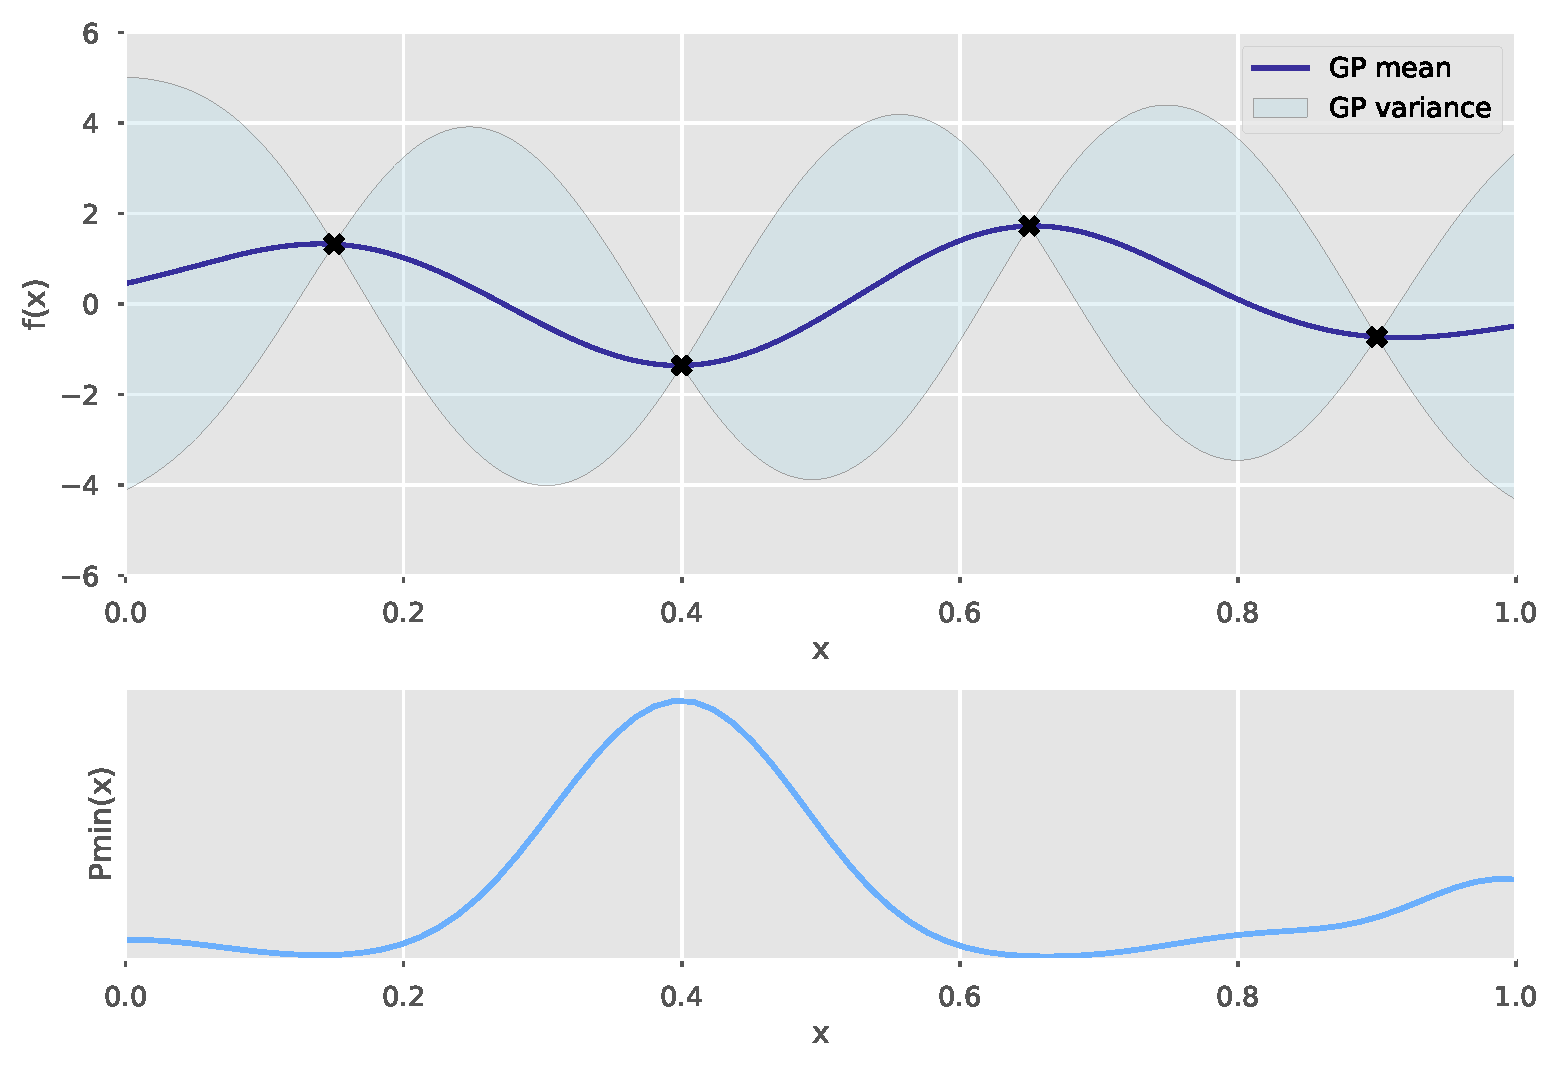
\includegraphics[width=0.7\textwidth, %height=0.4\textwidth]{images/intro_images/plot_posterior.pdf%}
%    \label{fig:my_label}
%\end{figure}
%\source{Plots are based on Javier Gonz\'alez's BO lecture (bo\_intro.py)}


%\end{frame}
%----------------------------------------------------------------------
\begin{frame}[c]{Introduction to Bayesian Optimization}
\framesubtitle{In a nutshell}

\begin{columns}[T]
\column{0.45\textwidth}
General approach
\begin{itemize}
    \item <2-> Fit a \emph{probabilistic model} to the collected function samples $\langle{}\conf, \cost(\conf)\rangle{}$
    \item <3-> Use the model to guide optimization, trading off \emph{exploration \vs{} exploitation}
%    \item Acquisition function for exploration-exploitation tradeoff
%    \item Optimize on acquisition function\\ to get next $x$ $\conf$ ($x$)
\end{itemize}

\onslide<11-> Popular approach in the statistics literature since \lit{\href{http://link.springer.com/chapter/10.1007\%2F3-540-07165-2_55}{Mockus et al. 1978}}
\begin{itemize}
    \item <12-> Efficient in \emph{\#function evaluations}
    \item <13-> Works when objective is \emph{nonconvex, noisy, has unknown derivatives, etc.}
    \item <14-> Recent \emph{convergence} results\\ \lit{\href{https://arxiv.org/abs/0912.3995}{Srinivas et al. 2009}; \href{http://www.jmlr.org/papers/v12/bull11a.html}{Bull et al. 2011}; \href{https://www.cs.ubc.ca/~nando/papers/BayesBandits.pdf}{de Freitas et al. 2012}; \href{http://papers.nips.cc/paper/5715-bayesian-optimization-with-exponential-convergence}{Kawaguchi et al. 2015}}
%    \item Popular \alert{Bayesian optimization workshop} at NIPS (the premiere machine learning conference)
\end{itemize}

\column{0.55\textwidth}
\onslide<1->
\begin{figure}
    \centering
    \only<1>{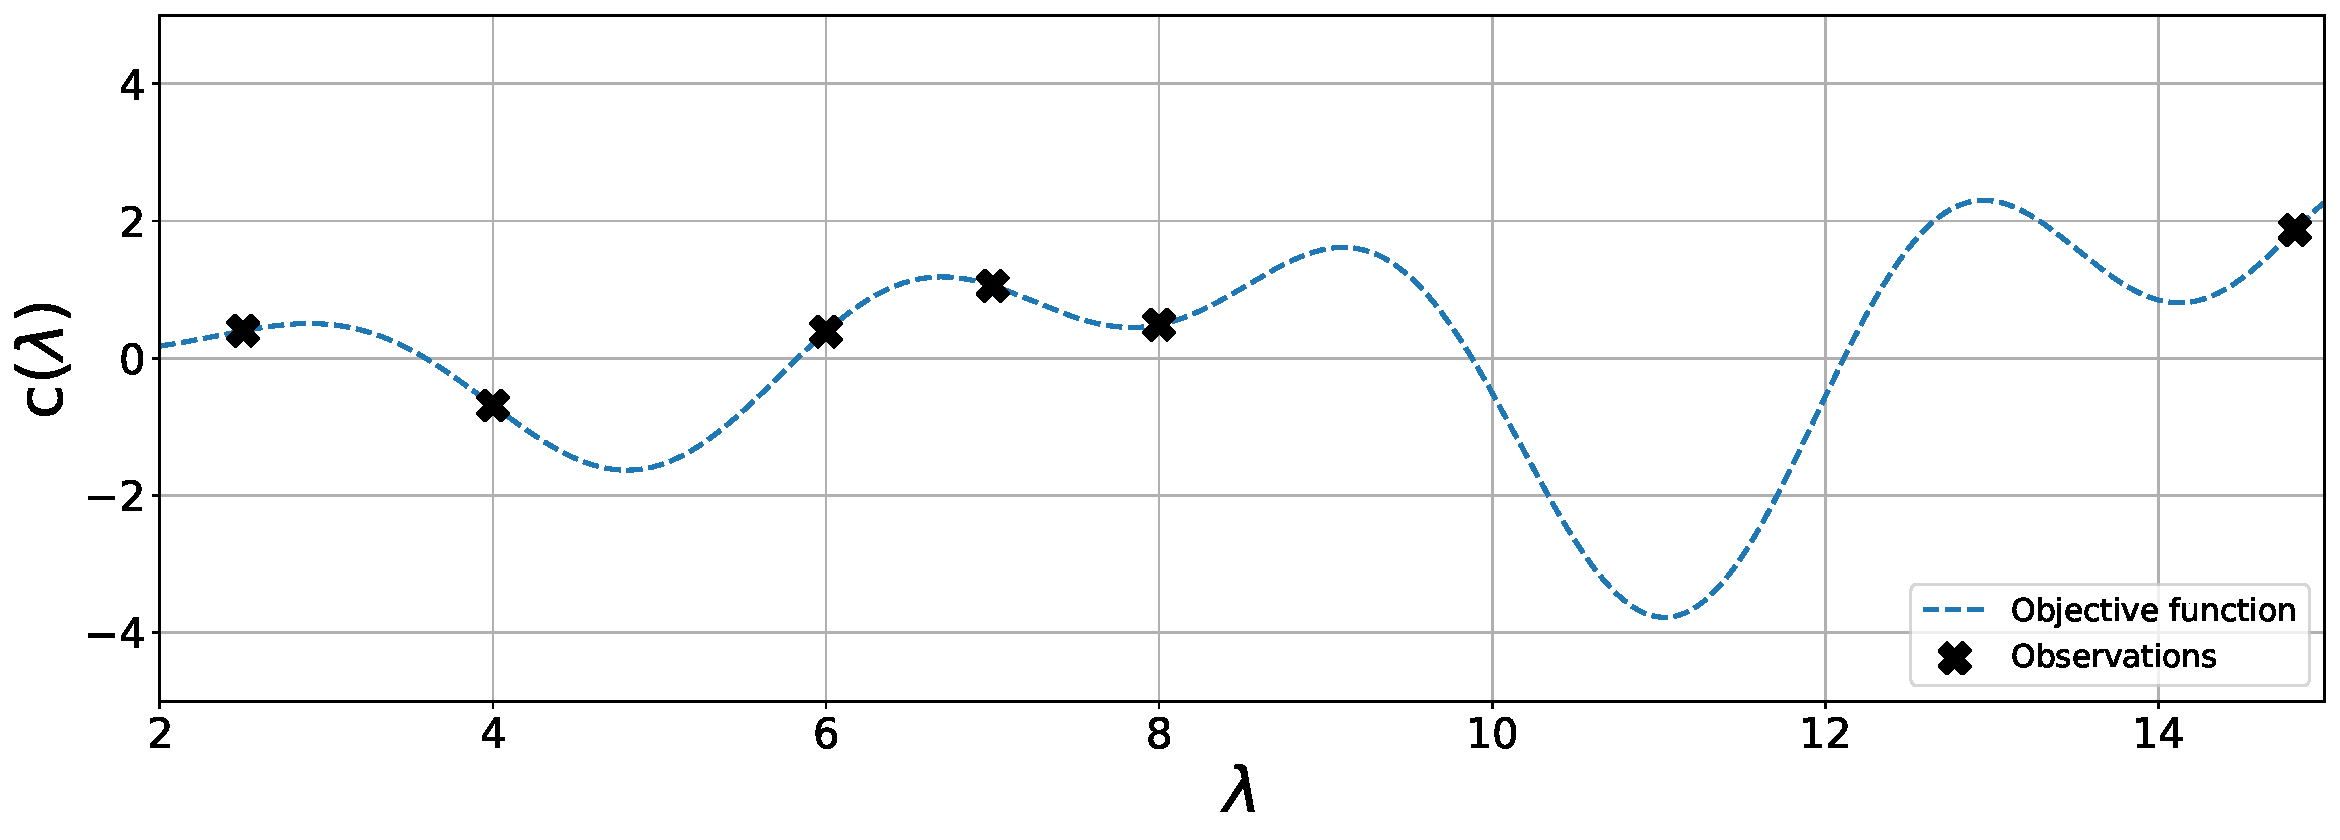
\includegraphics[width=\textwidth]{images/intro_images/BOLoop_Initial_Points.pdf}}
    \only<2>{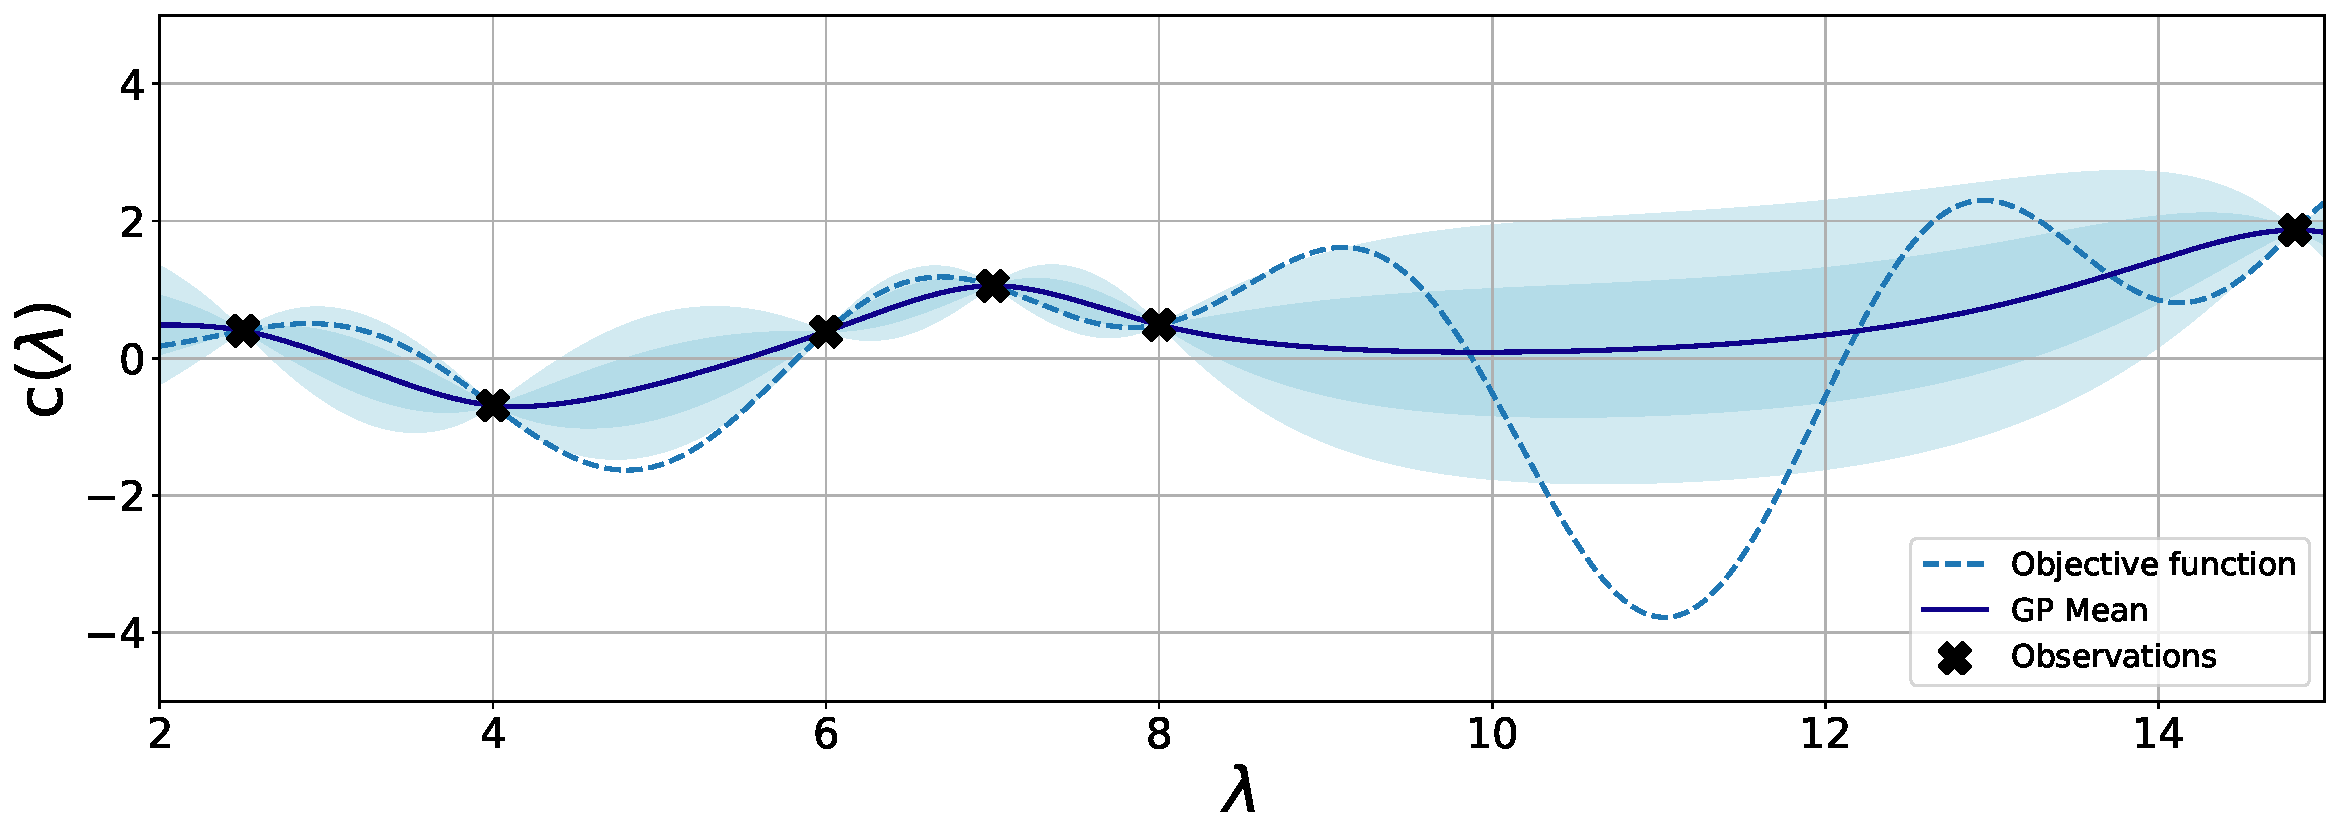
\includegraphics[width=\textwidth]{images/intro_images/BOLoop_Initial_Points_and_GP.pdf}}
    \only<3>{\includegraphics[width=\textwidth]{images/intro_images/plot_1.pdf}}
    \only<4>{\includegraphics[width=\textwidth]{images/intro_images/plot_2.pdf}}
    \only<5>{\includegraphics[width=\textwidth]{images/intro_images/plot_3.pdf}}
    \only<6>{\includegraphics[width=\textwidth]{images/intro_images/plot_4.pdf}}
    \only<7>{\includegraphics[width=\textwidth]{images/intro_images/plot_5.pdf}}
    \only<8>{\includegraphics[width=\textwidth]{images/intro_images/plot_6.pdf}}
    \only<9->{\includegraphics[width=\textwidth]{images/intro_images/plot_7.pdf}}
\end{figure}
\end{columns}

\end{frame}
%-----------------------------------------------------------------------
%\myframe{Bayesian Optimization in a Nutshell}{
%  
%\vspace*{-0.5cm}
%\begin{columns}[T]
%
%\column{0.6\textwidth}
%
%\myblock{General approach}{
%	\myit{
%	  \item Fit a probabilistic model to the collected function samples
%	  $\langle{}\conf, \cost(\conf)\rangle{}$
%	  \item Use the model to guide optimization, trading off
%	  exploration \vs{} exploitation
%	%  \item Acquisition function for exploration-exploitation tradeoff
%	%  \item Optimize on acquisition function\\ to get next $x$
%	  %$\conf$ ($x$)
%	}
%}
%
%\smallskip
%\onslide<5->{
%	\myblock{Popular approach in the statistics literature since \litw{\href{http://link.springer.com/chapter/10.1007\%2F3-540-07165-2_55}{Mockus,
%	1978}}}{ \myit{
%		  	\item Efficient in \# function evaluations 
%		  	\item Works when objective is nonconvex, noisy, has unknown derivatives, etc
%			\pause
%			\item Recent convergence results\\ \lit{Srinivas et al, 2010; Bull 2011;
%			de Freitas et al, 2012; Kawaguchi et al, 2015}
%			%TODO: sorry, I don't know these papers
%		%	\item Popular \alert{Bayesian optimization workshop} at NIPS (the premiere machine learning conference)
%		}
%	}
%}
%%\begin{enumerate}
%%  \item Fit an empirical performance model (EPM) 
%%  \item Acquisition function for exploration-exploitation tradeoff
%%  \item Optimize on acquisition function\\ to get next $\conf$ ($x$)
%%\end{enumerate}
%
%\column{0.4\textwidth}
%\vspace*{0.5cm}
%\onslide<2->{
%	%\includegraphics[width=1\textwidth]{../images/bo.png}
%	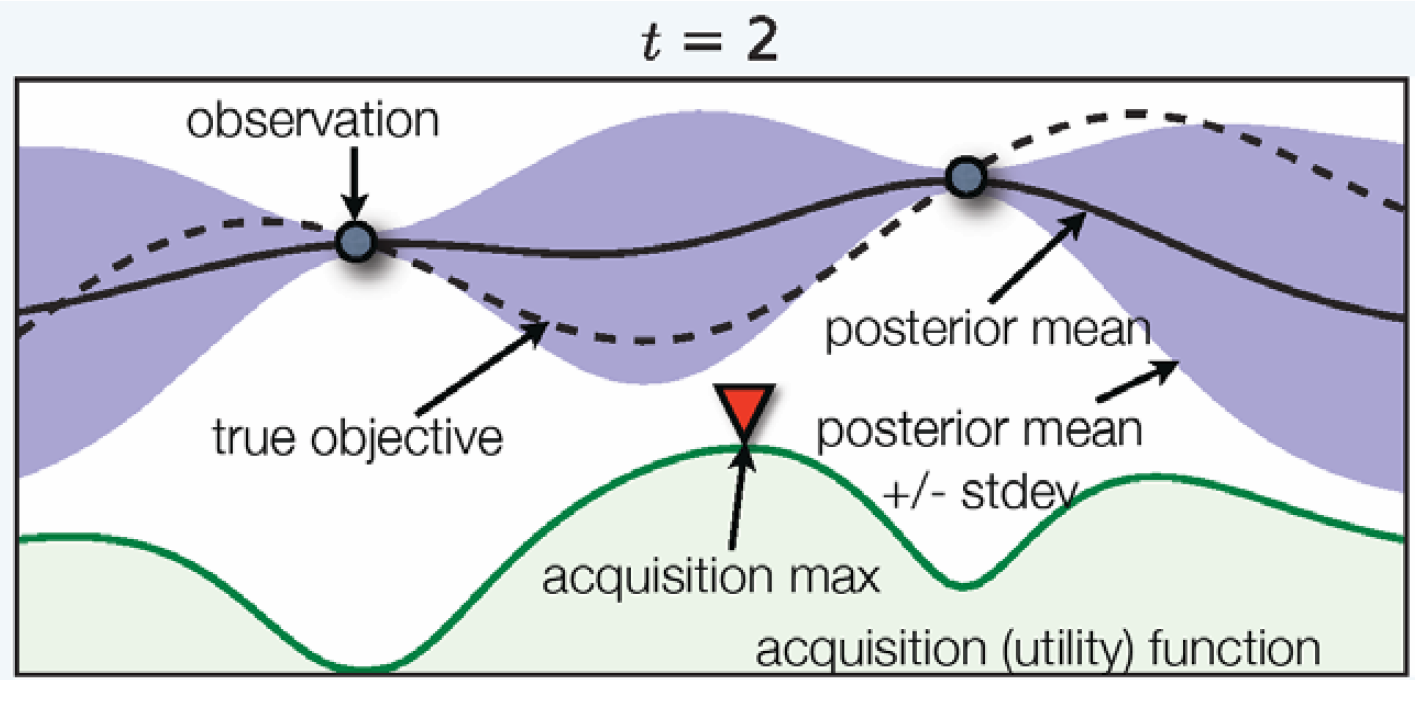
\includegraphics[width=0.9\textwidth]{plots_and_scripts/plots/bo_pic1.png}\\
%	\pause
%	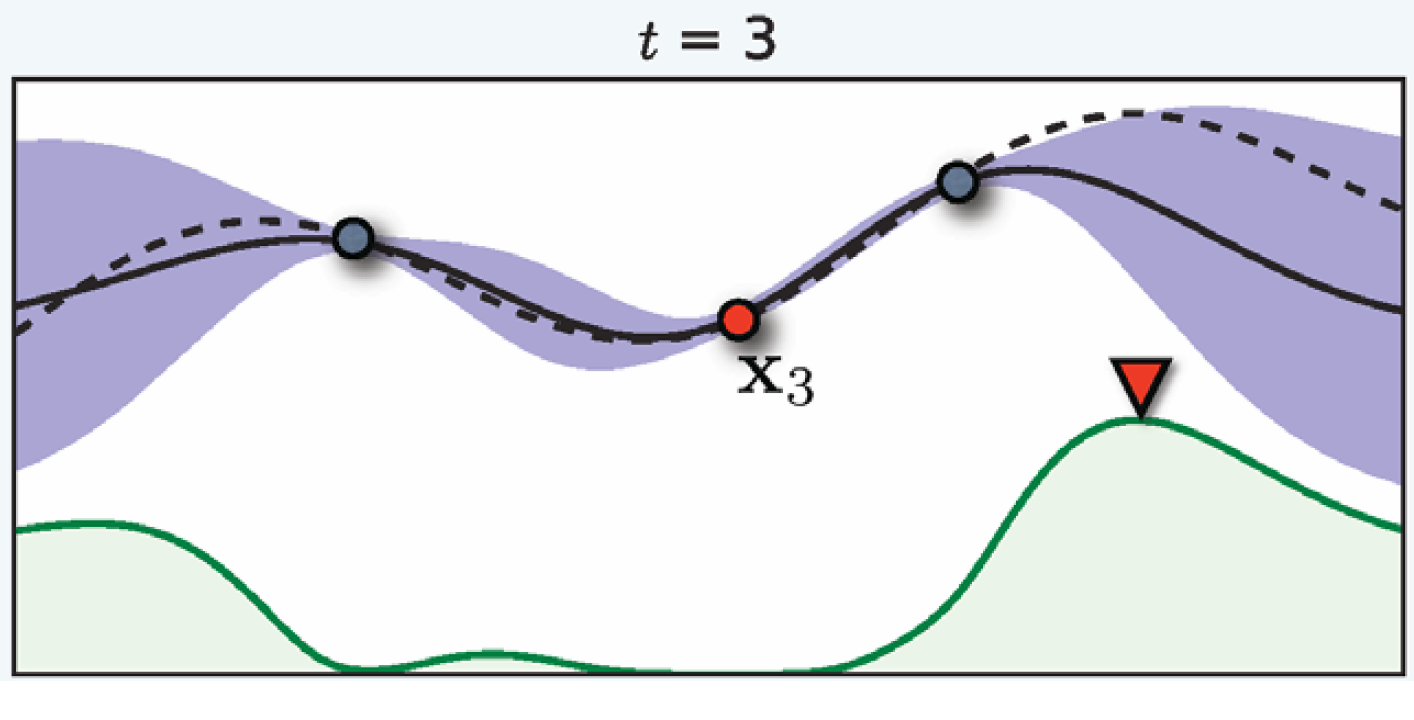
\includegraphics[width=0.9\textwidth]{plots_and_scripts/plots//bo_pic2.png}\\
%	\pause
%	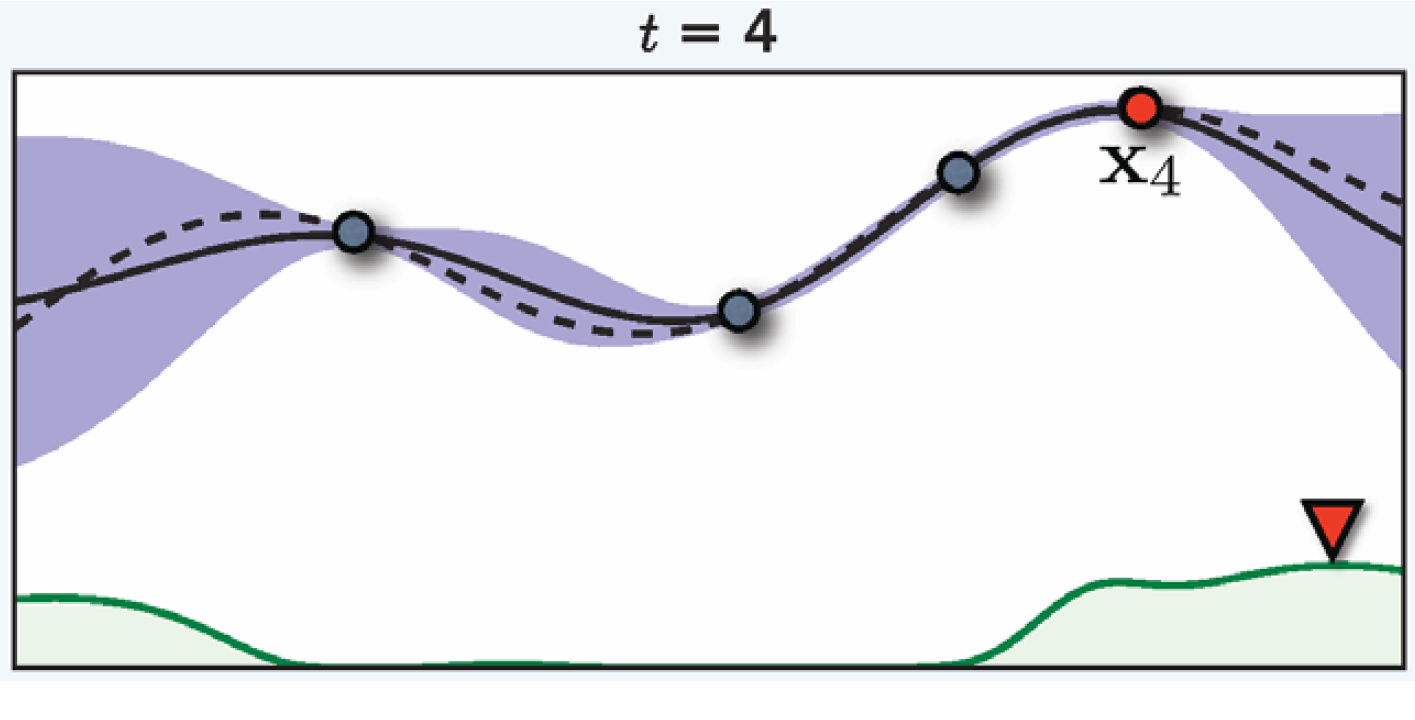
\includegraphics[width=0.9\textwidth]{plots_and_scripts/plots//bo_pic3.png}\\
%	\footnotesize{Image source: \lit{\href{https://arxiv.org/abs/1012.2599}{Brochu et al, 2010}}}
%}
%\end{columns}
%}
%----------------------------------------------------------------------
%5\begin{frame}[c]{Bayesian Optimization: Visualization of Many Steps}
%\begin{figure}
%    \centering
%    \only<1>{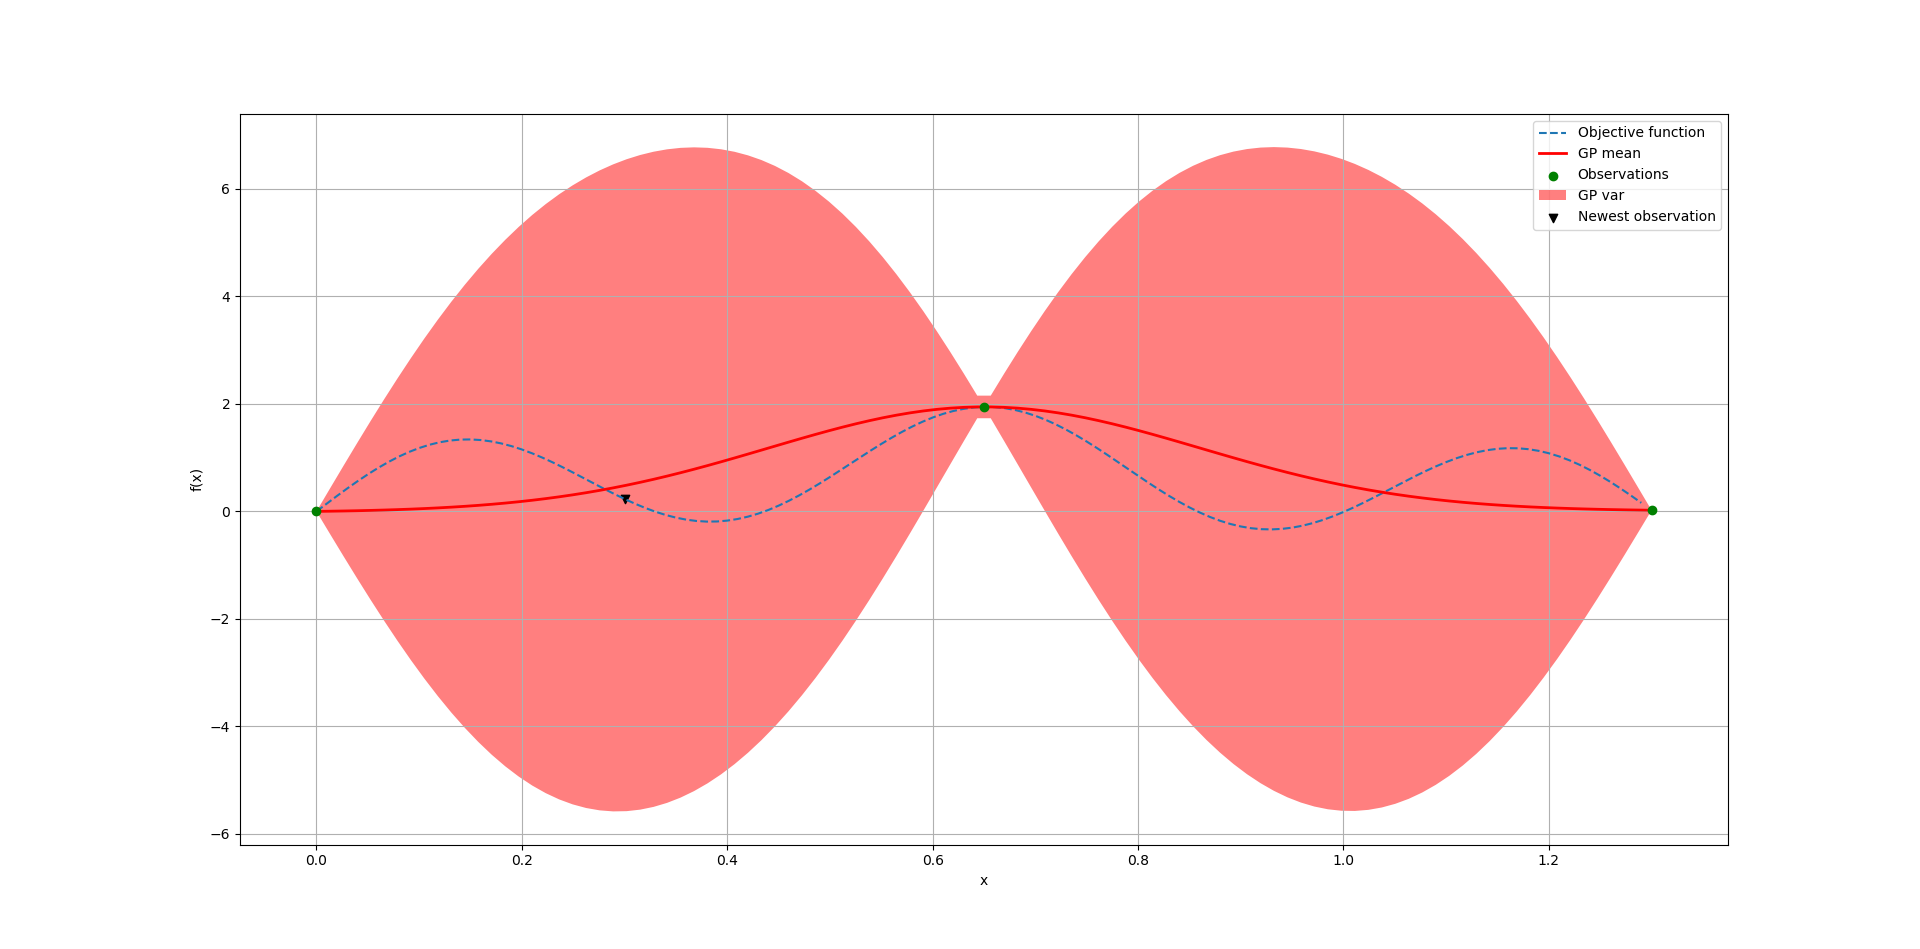
\includegraphics[width=\linewidth]{images/intro_images/BOLoop_1.png}}
%    \only<2>{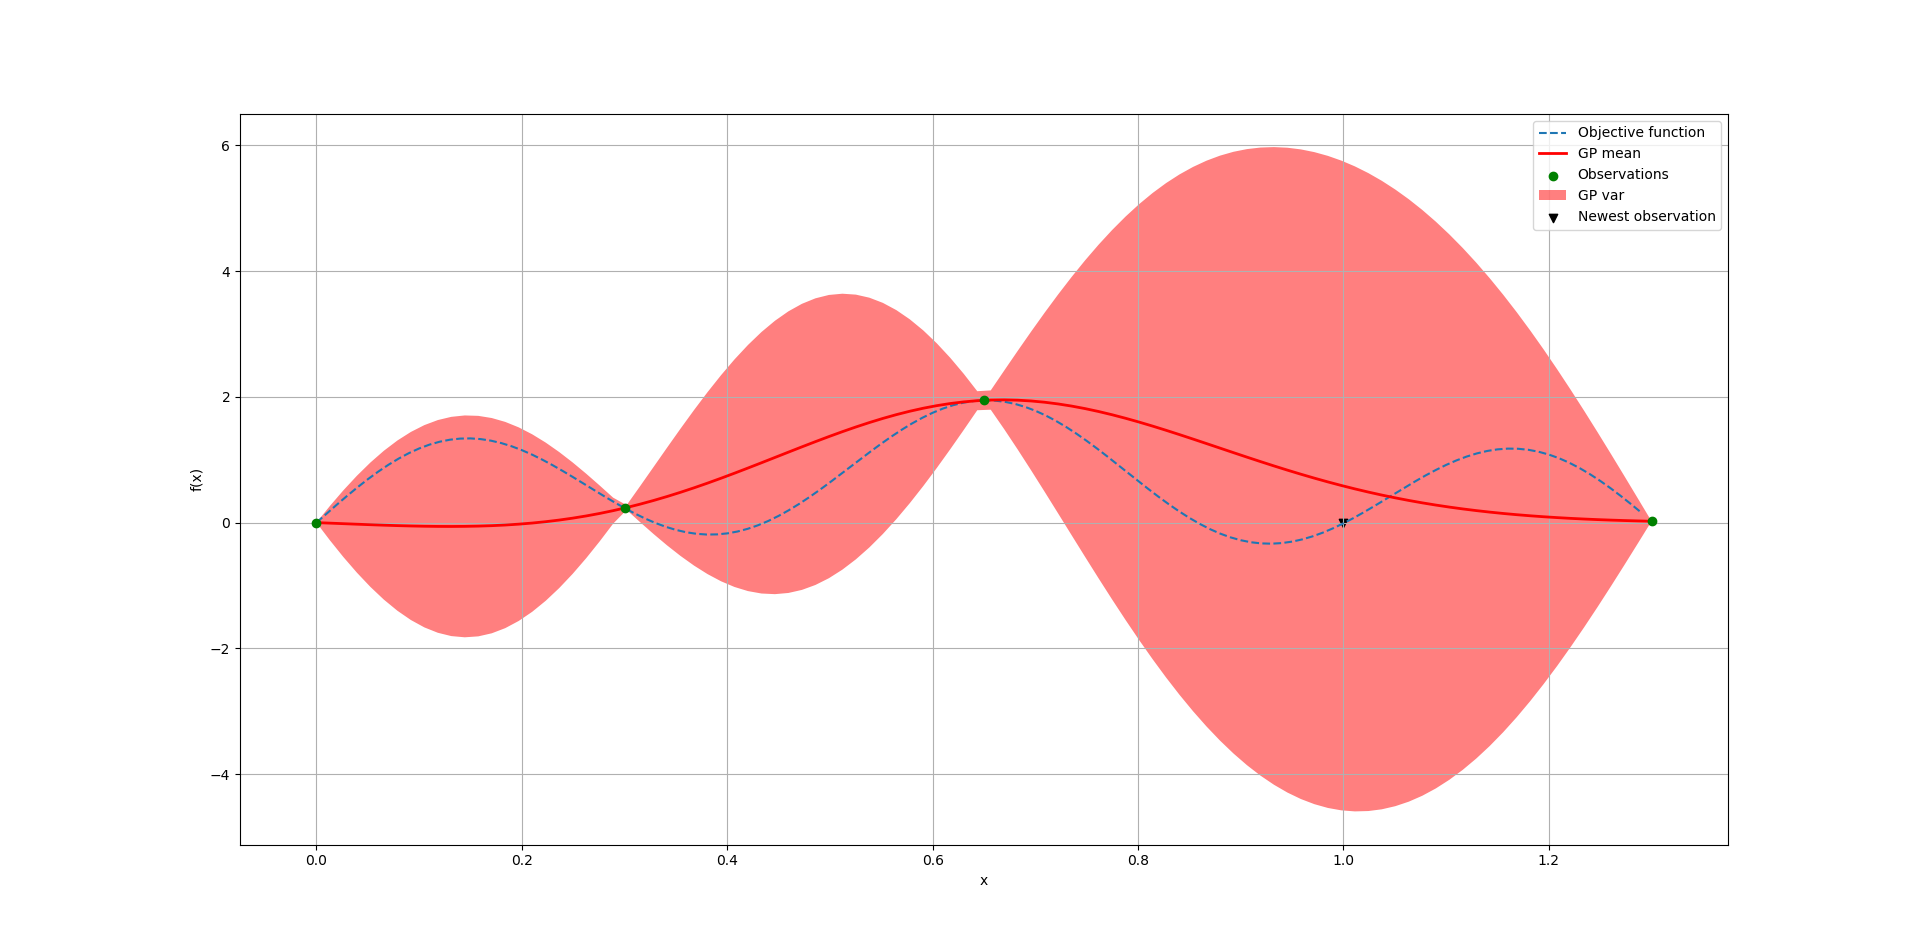
\includegraphics[width=\linewidth]{images/intro_images/BOLoop_2.png}}
%    \only<3>{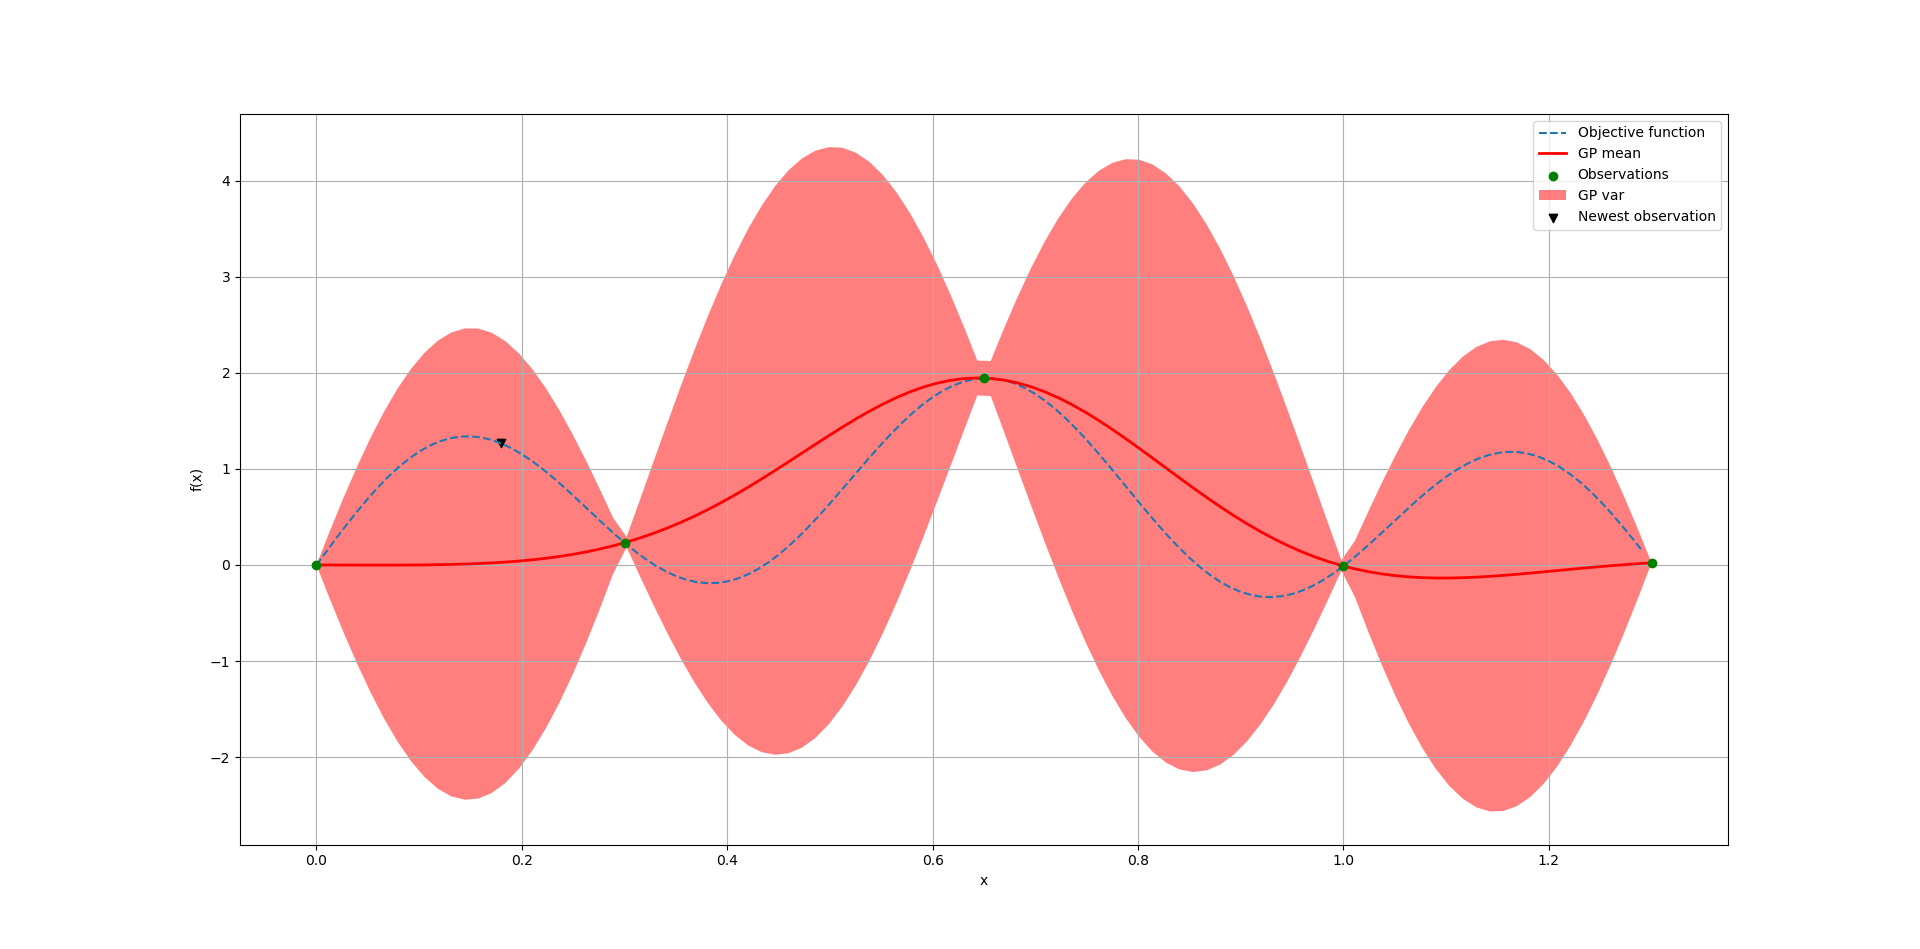
\includegraphics[width=\linewidth]{images/intro_images/BOLoop_3.png}}
%    \only<4>{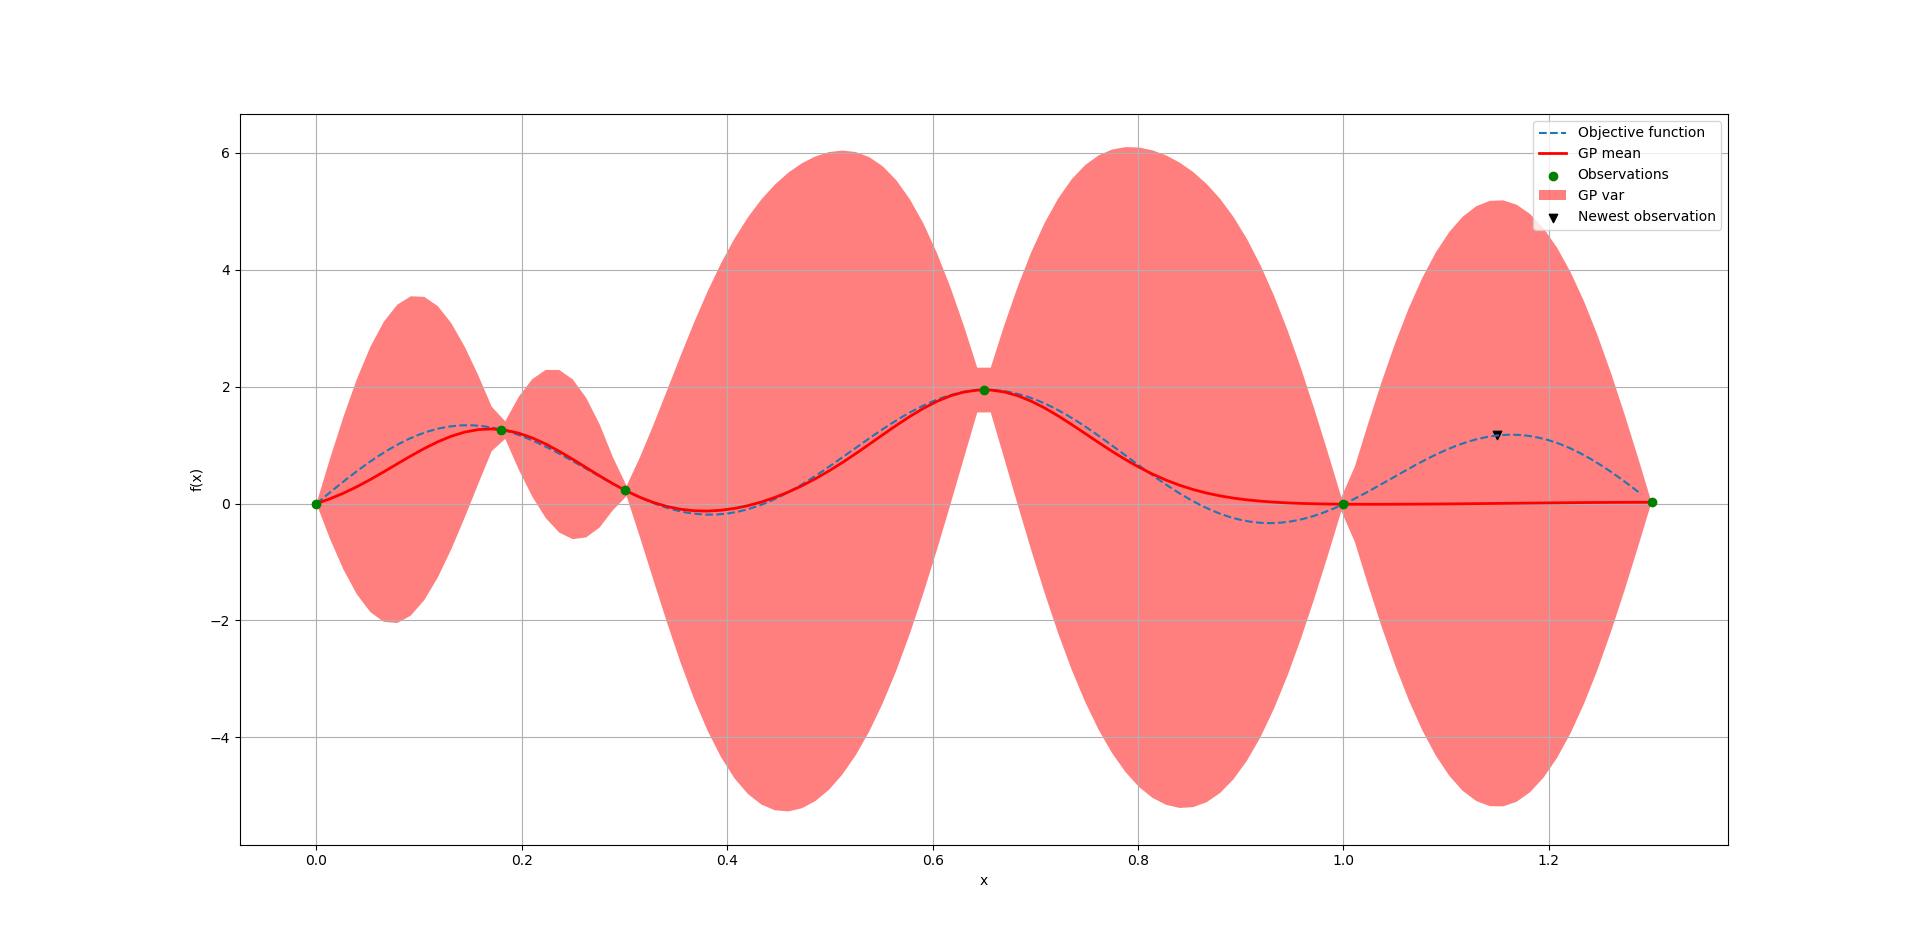
\includegraphics[width=\linewidth]{images/intro_images/BOLoop_4.png}}
%    \only<5>{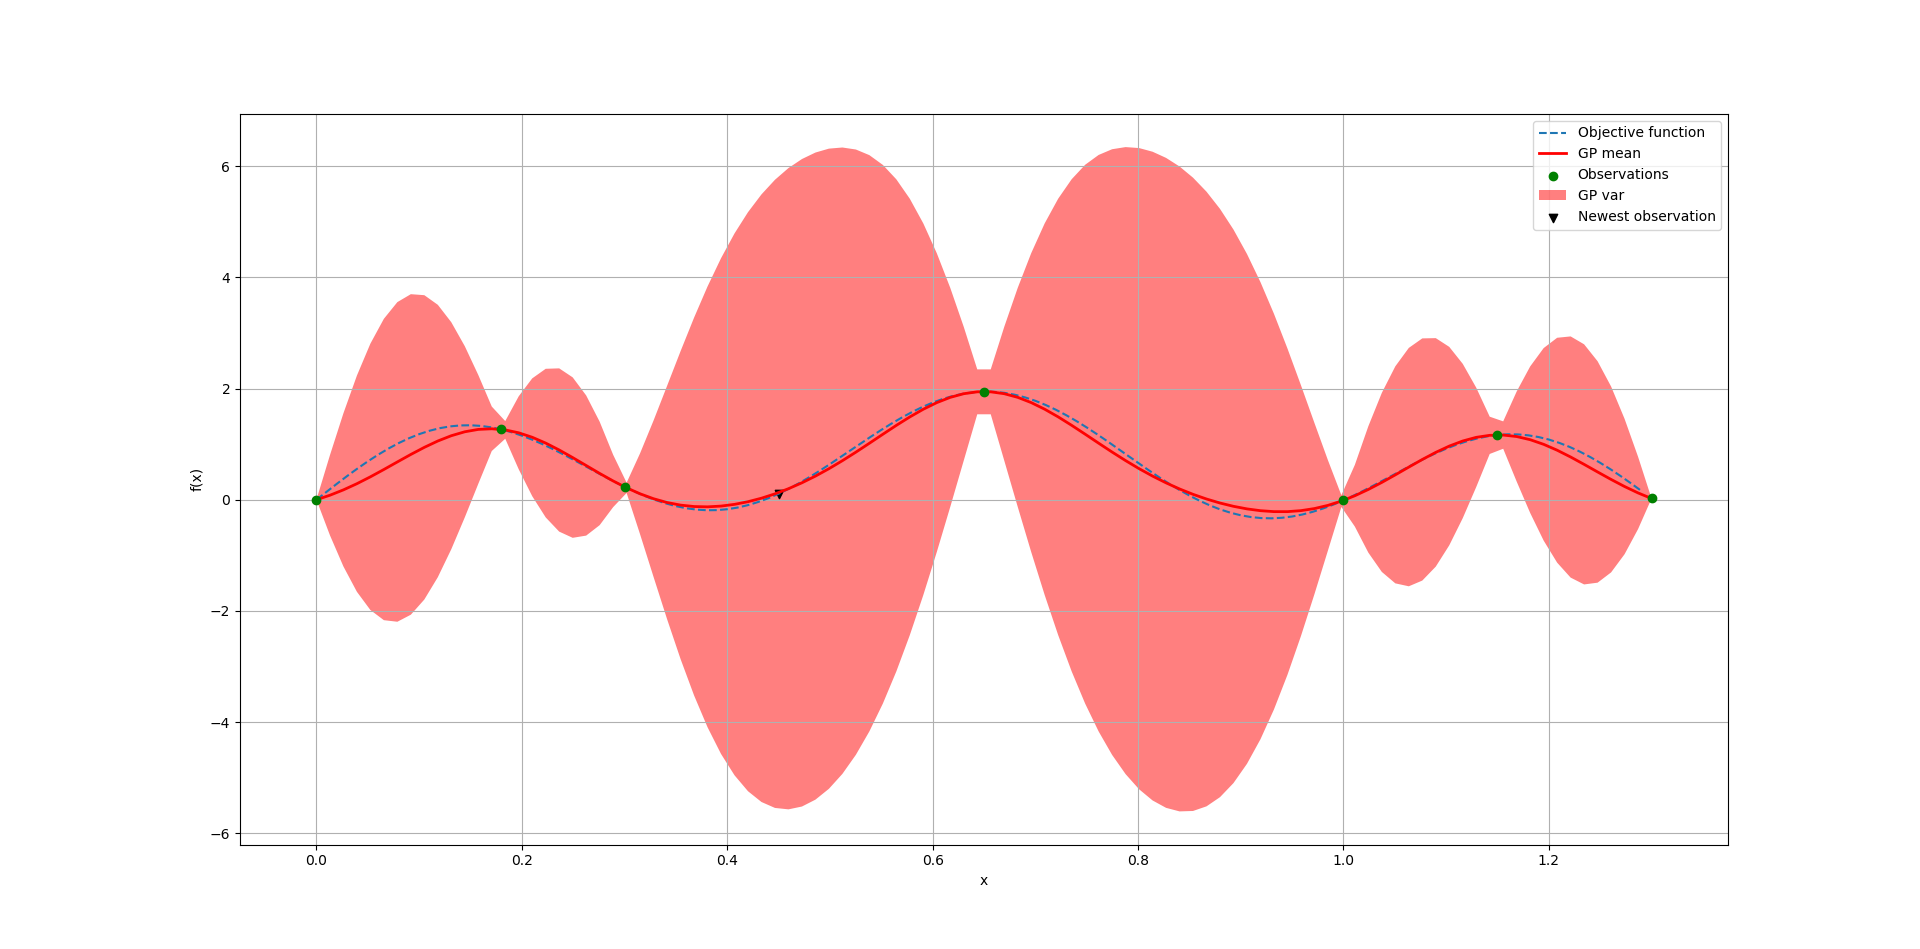
\includegraphics[width=\linewidth]{images/intro_images/BOLoop_5.png}}
%    \only<6>{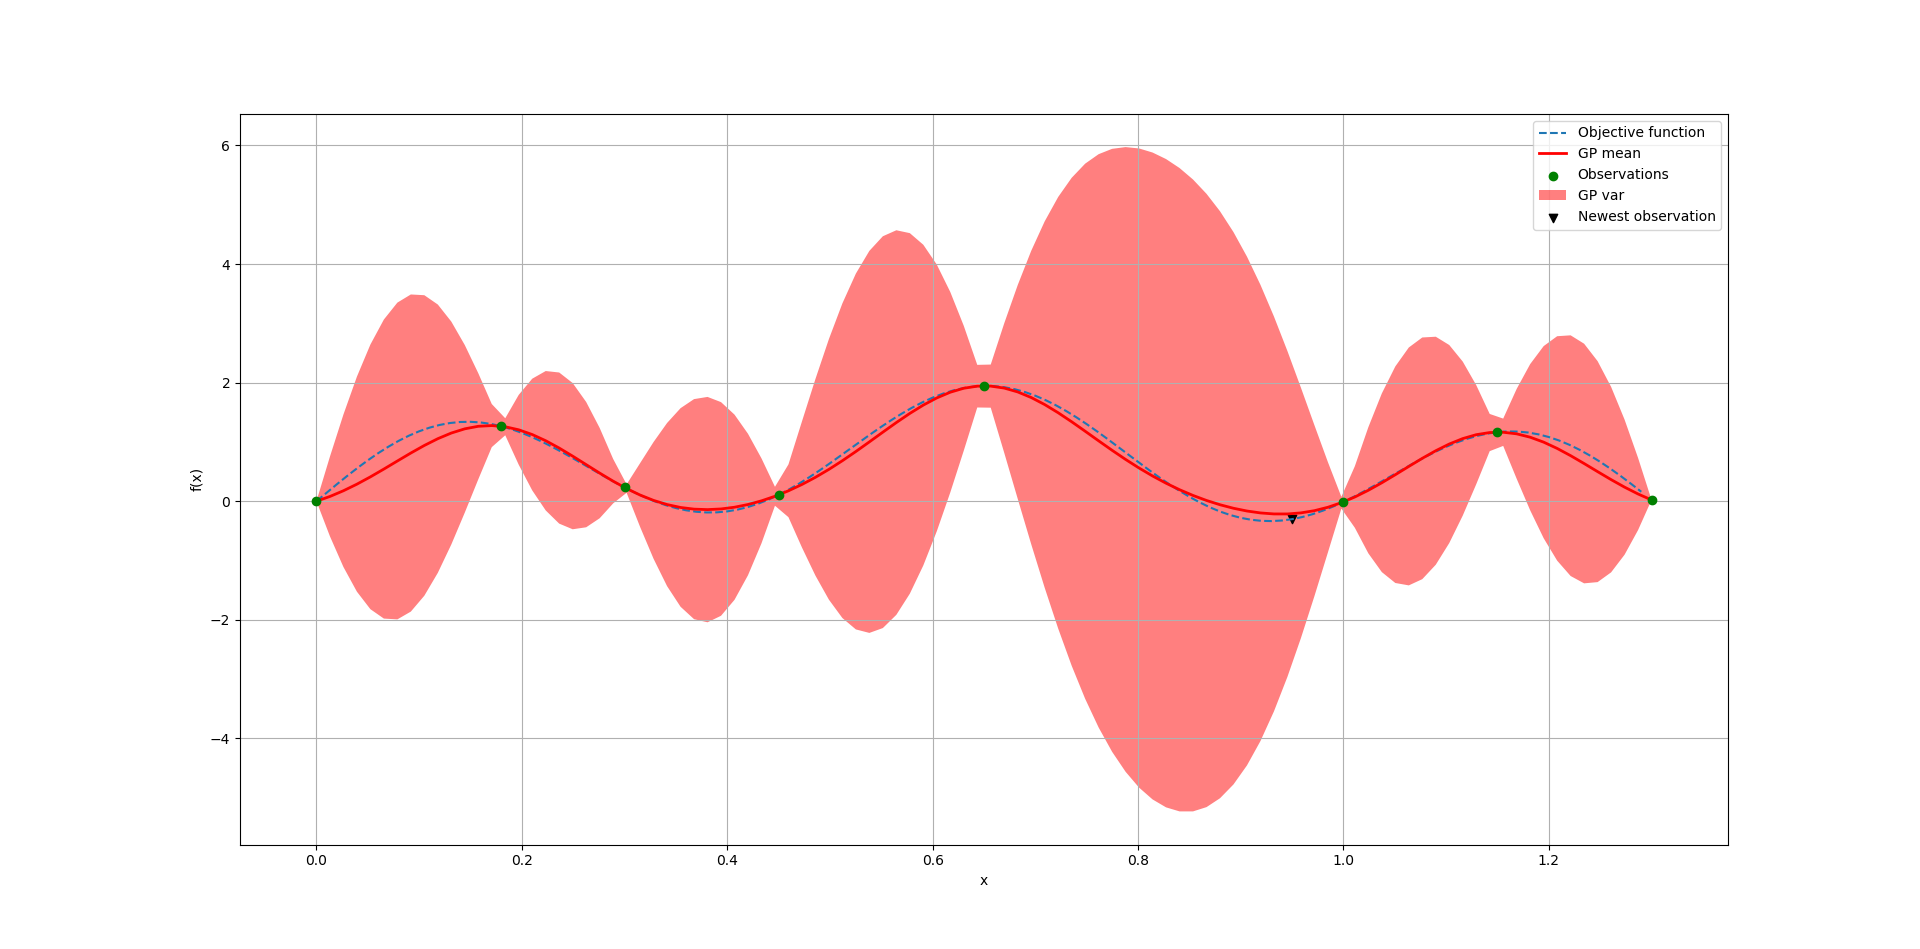
\includegraphics[width=\linewidth]{images/intro_images/BOLoop_6.png}}
%    \only<7>{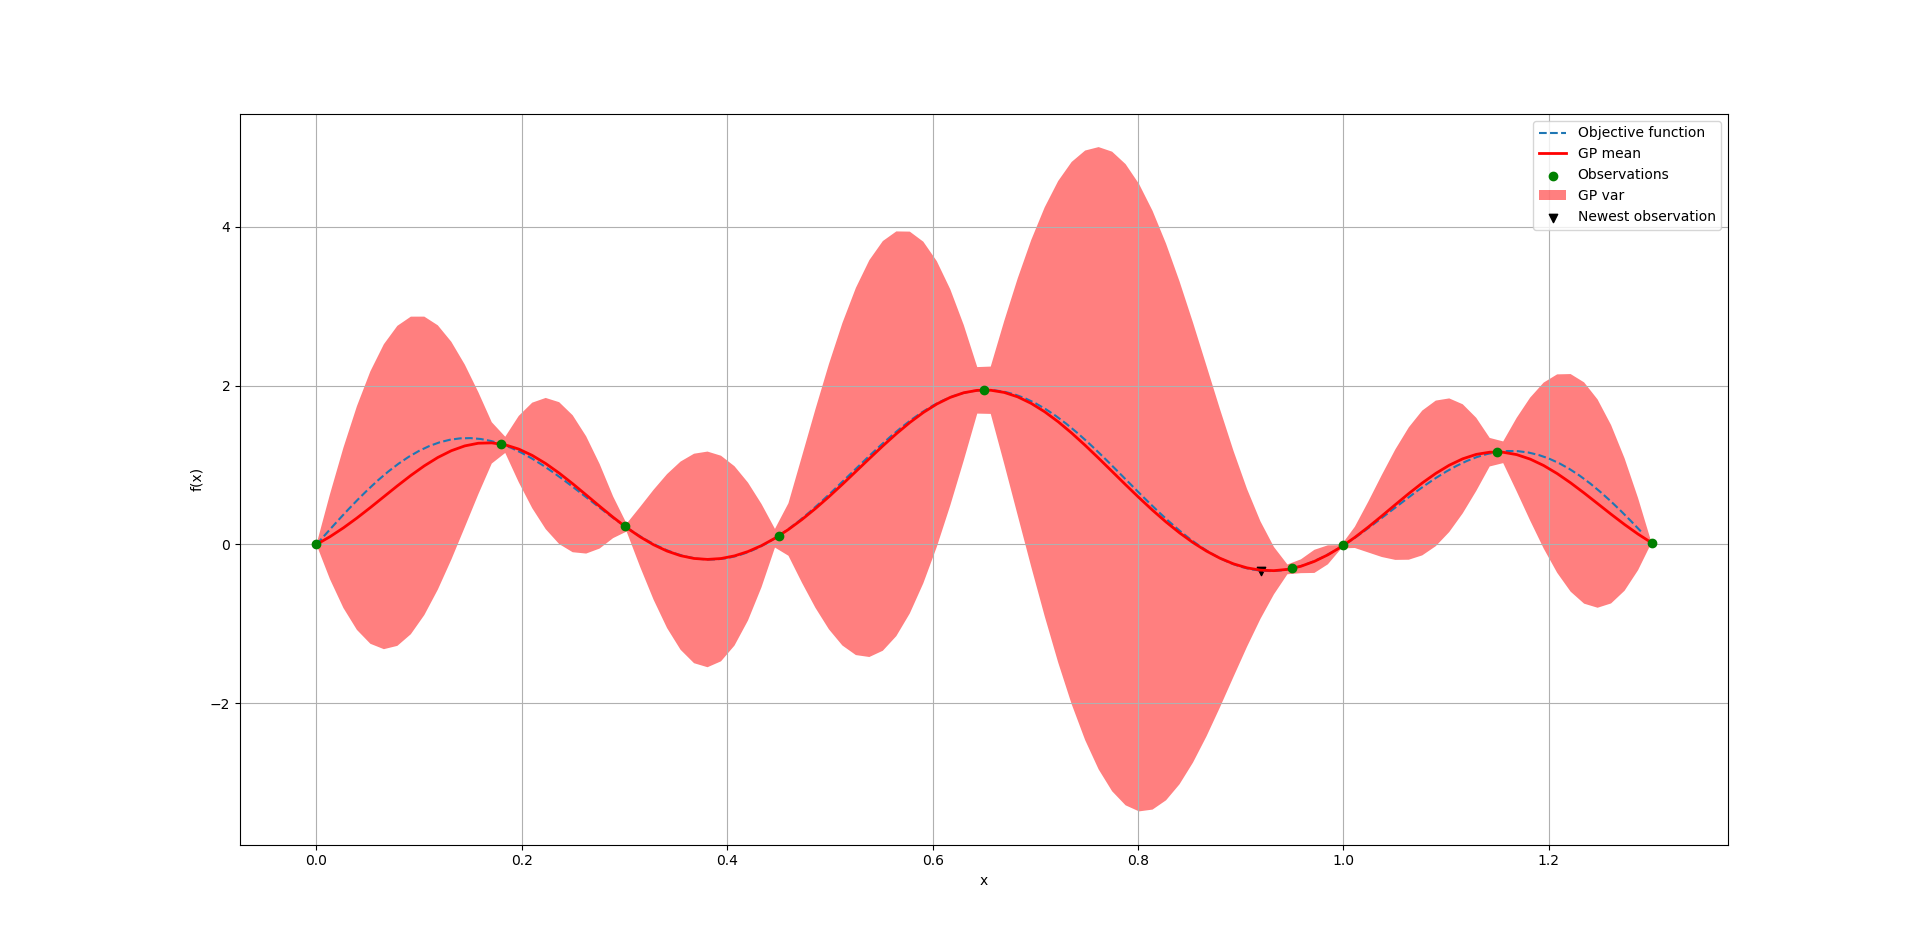
\includegraphics[width=\linewidth]{images/intro_images/BOLoop_7.png}}
%    \only<8>{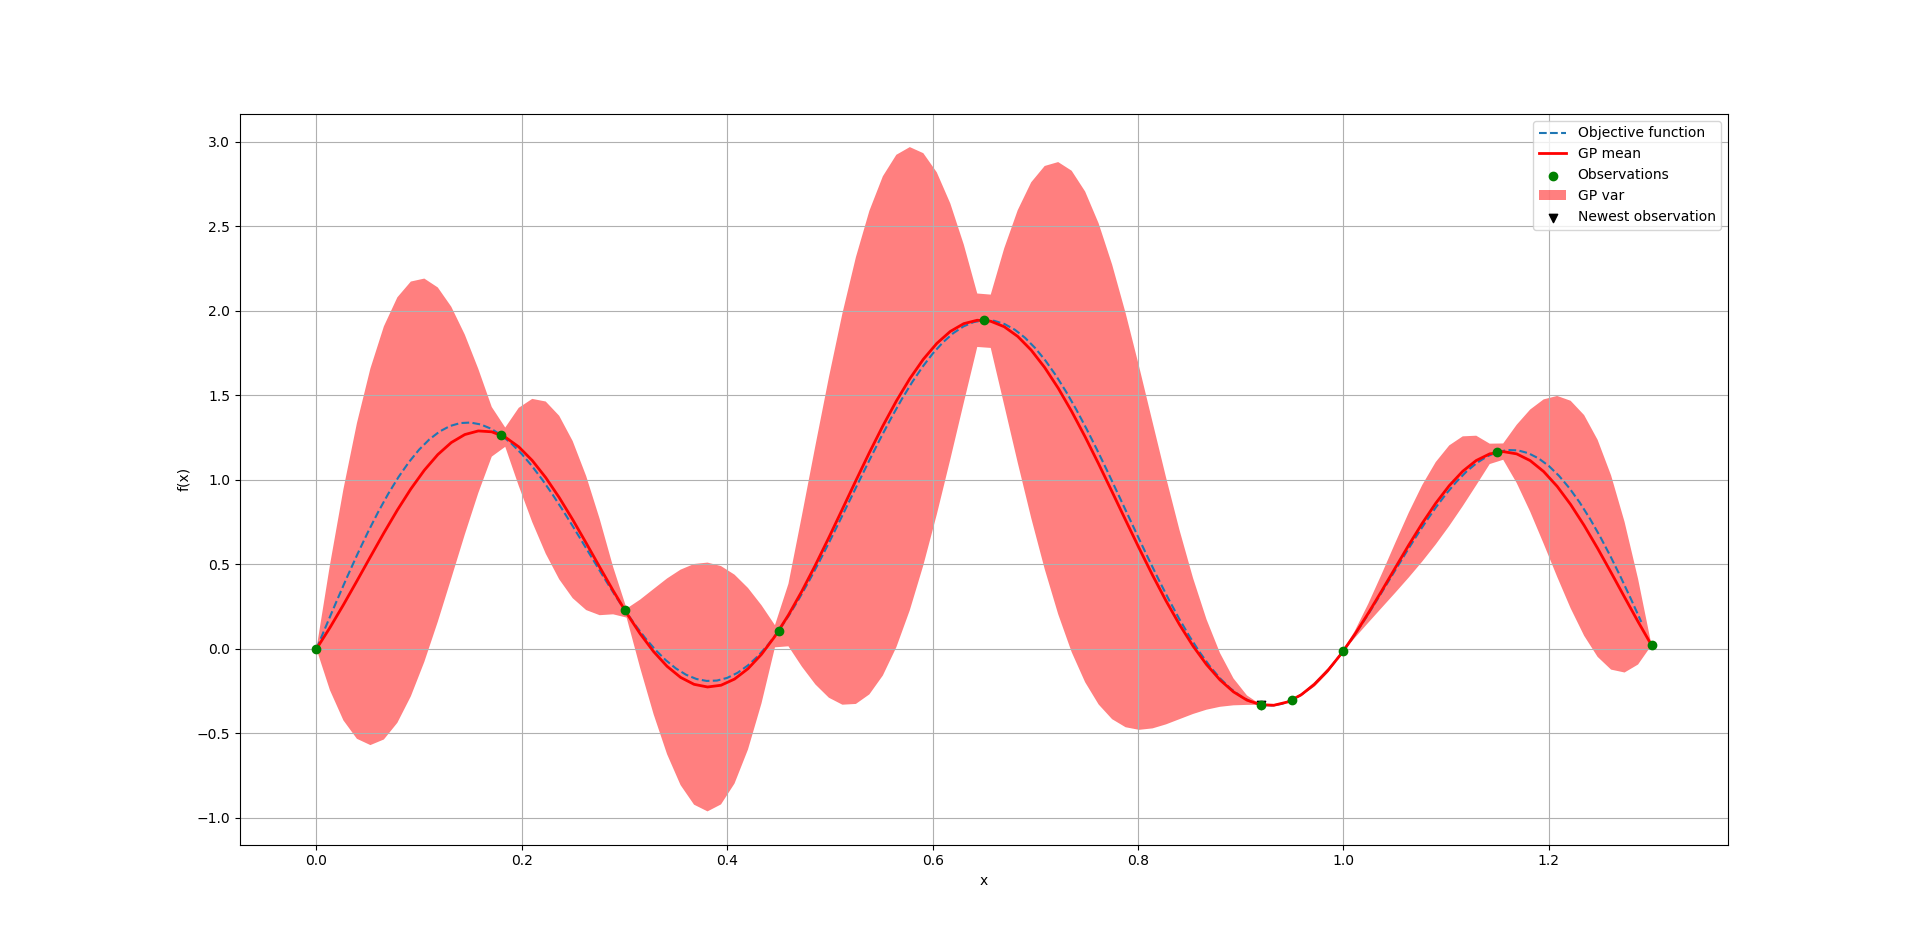
\includegraphics[width=\linewidth]{images/intro_images/BOLoop_8.png}}
%\end{figure}
%\end{frame}
%----------------------------------------------------------------------

\begin{frame}[c]{Introduction to Bayesian Optimization}
\framesubtitle{Pseudocode}

\begin{center}
\begin{minipage}{0.75\textwidth}
\begin{algorithm}[H]
    %\DontPrintSemicolon
    \SetAlgoLined
    \setcounter{AlgoLine}{0}
    \SetKwInOut{Require}{Require}
    \SetKwInOut{Result}{Result}
    
    \Require{Search space $\pcs$, 
    		cost function $\cost$, 
    		acquisition function $\acq$, predictive model $\surro$,
    		maximal number of function evaluations $\bobudget$}
    \Result{Best observed configuration $\finconf$ according to $\iter[\bobudget]{\dataset}$ or $\surro$}
    
	$\iter[0]{\dataset} \leftarrow \varnothing$\; 
	 
    \For{$\bocount=1$ \KwTo $\bobudget$}{
		%\While{$B$ not exhausted} {
		$\iter[\bocount]{\surro}$ $\leftarrow$ fit predictive model on $\iter[\bocount-1]{\dataset}$\;
		
		$\bonextsample \leftarrow \bonextsample \in \argmax_{\conf \in \pcs} \acq(\conf; \iter[\bocount-1]{\dataset}, \iter[\bocount]{\surro})$\;
		
		Query $\bonextobs$\;
		
		$\iter[\bocount]{\dataset} \leftarrow \iter[\bocount-1]{\dataset} \cup \{\langle \bonextsample, \bonextobs \rangle \}$\;
	}
	\caption{BO loop}
\end{algorithm}
\end{minipage}
\end{center}
\end{frame}
%-----------------------------------------------------------------------
\begin{frame}[c]{Introduction to Bayesian Optimization}
\framesubtitle{Where does the name come from?}

\begin{itemize}
    \item <+-> Bayesian optimization uses Bayes' theorem: 
    	\begin{equation*}
    	    P(A \vert B) = \frac{P(B \wedge A) \times  P(A)}{P(B)}
    	    \propto P(B \vert A) \times  P(A)
    	\end{equation*} 
    \item <+-> We refer to:
        \begin{itemize}
            \item $A$ as a model (or hypothesis, theory), 
            \item $B$ as a data (or observations, evidence),
            \item $P(A \vert B)$ as a \emph{posterior} probability of a model given a data,
            \item $P(B \vert A)$ as a \emph{likelihood} of a data given a model, 
            \item $P(A)$ as a \emph{prior} probability of a model, which represents our belief about the space of possible objective functions. 
        \end{itemize}
    \item <+-> In our application:
        \begin{equation*}
            P(\func \vert \dataset_{1:\bocount}) \propto P(\dataset_{1:\bocount} \vert \func) \times P(\func)
        \end{equation*} 
        where $\dataset_{1:\bocount} = \left \{ \conf_{1:\bocount}, \cost(\conf_{1:\bocount}) \right \}$.
\end{itemize}
\end{frame}
%-----------------------------------------------------------------------
\begin{frame}[c]{Introduction to Bayesian Optimization}
\framesubtitle{Advantages and Disadvantages}

\begin{columns}[T] % align columns
\begin{column}{.48\textwidth}


\begin{block}{Advantages}
\begin{itemize}
  \item Sample efficient 
  \item Can handle noise
  \item Native incorporation of priors 
  \item Does not require gradients 
  \item Theoretical guarantees
\end{itemize}
\end{block}

\end{column}%

\hfill%
\pause 
\begin{column}{.48\textwidth}

\begin{block}{Disadvantages}
\begin{itemize}
  \item Overhead because of model training in each iteration 
  \item Open design choices: surrogate model, acquisition function
  \item Inherently sequential (in its basic form)
\end{itemize}
\end{block}

\end{column}
\end{columns}

\end{frame}
%-----------------------------------------------------------------------
\begin{frame}[c]{Learning Goals of this Lecture}

\begin{enumerate}
    \item Learn how Bayesian optimization works and can be used for HPO.
    \item Learn about the two main ingredients of Bayesian optimization: Acquisition Functions and Surrogate Models.
    \item Learn the limits of Bayesian optimization and the extensions which tackle these.
    \item Know success stories of Bayesian optimization.
\end{enumerate}

\end{frame}

%-----------------------------------------------------------------------
%----------------------------------------------------------------------
%\begin{frame}[c]{Surrogate modelling}
%\framesubtitle{General idea}
%\begin{itemize}
%    \item Use a surrogate model of the expensive function $\cost$ as a cheap-to-evaluate proxy.
%    \begin{itemize}
%        \item Use a probabilistic model with well-calibrated uncertainty predictions.
%    \end{itemize}
%    \pause
%    \item Define a utility function to guide the search for new data points.
%    \pause
%    \item Use the optimization of the utility function as a decision procedure to provide inference on where to evaluate next.
%
%\end{itemize}
%\end{frame}

%-----------------------------------------------------------------------
